% !TEX TS-program = pdflatexmk
\documentclass[11pt]{article}
\usepackage[margin=1in]{geometry} 
\usepackage[parfill]{parskip}% Begin paragraphs with an empty line rather than an indent
\usepackage{graphicx}
\usepackage{booktabs}
\pdfmapfile{+zi4.map}
%SetFonts
% libertine text and newtxmath
%\usepackage{lmodern}
\usepackage[lining]{libertine}
\usepackage[T1]{fontenc}
%\usepackage[scaled=.83]{beramono}
\usepackage[varqu]{zi4}
%\usepackage{amsmath,amsthm}
\usepackage[libertine,cmbraces]{newtxmath}
\usepackage{textcomp}
\renewcommand\rmdefault{LinuxLibertineT-OsF}
\usepackage[supstfm=libertinesups,%
  supscaled=1.2,%
  raised=-.13em]{superiors}
%SetFonts
%\UndeclareTextCommand{\textquotesingle}{LY1}
%\DeclareTextSymbol{\textquotesingle}{TS1}{39}
%\usepackage{upquote}
\title{The Inconsolata  Package}
\author{Michael Sharpe}
\date{\today}  % Activate to display a given date or no date

\begin{document}
%\show\textquotesingle
\maketitle
The package provides support files for the typewriter font
\texttt{Inconsolata}. To use it add \verb|\usepackage{zi4}| to your document. This
will change the typewriter font family to \texttt{zi4}, the family name used
by this package, which replaces the old \textsf{inconsolata}, where the family name was \texttt{fi4}. The package also provides extensions of the \texttt{Inconsolata} fonts in regular and bold weights, adding some glyphs which may optionally replace existing \texttt{quotedbl} and \texttt{quotesingle} and lower-case~L, along with new \texttt{arrowright} and \texttt{arrowleft} glyphs. As with Karl Berry's original \texttt{inconsolata} package, the \LaTeX\ package \texttt{zi4} offers four encodings---\texttt{T1}, \texttt{LY1}, \texttt{OT1} and \texttt{QX}---and provides the following options which some may find improve its utility for displaying verbatim text such as code fragments. 
\begin{itemize}
\item The option \texttt{scaled=x} allows you to scale all typewriter text and verbatim text by the factor \texttt{x}.
\item
The default zero in \texttt{zi4} is now slashed. The unslashed zero may be specified with the option \texttt{var0}.
\item For those who find the default lower-case L(\texttt{l}) a bit too close to the numeral~\texttt{1}, there is an option \texttt{varl} which substitutes a more distinctive shape for all glyphs related to lower-case L.
\item The \texttt{zi4} package loads the \texttt{textcomp} package, which points to a TS$1$-encoded font that has been modified to have uncurved left and right quotes, especially important in code fragments, by use of \texttt{textcomp} glyphs \verb|\textasciigrave| and \verb|\textquotesingle|. The \texttt{varqu} option provides further upright quote forms for glyphs that are not part of the \texttt{textcomp} package, such as 
the default double quote glyph \texttt{quotedbl} and \texttt{quotesingle}, which by default have a small slant. (Note that the latter is not part of all encodings---it is present in \texttt{OT1}, \texttt{LY1} and \texttt{QX}, but not in \texttt{T1}.)
\item The package loads \texttt{upquote} by default, but provides an option \texttt{noupquote} to override it.
\end{itemize}
When used in ordinary typewriter mode (ie, with \verb|\texttt{}| or the deprecated form \verb|{\tt }|), left and right quotes are rendered as in ordinary text. For example, 
\begin{verbatim}
\texttt{`xy' " \textasciigrave \textquotesingle}
\end{verbatim}
renders (with option \texttt{varqu}) as \texttt{`xy' " \textasciigrave \textquotesingle}. With the \texttt{upquote} package, verbatim text, eg:
\begin{verbatim}
\verb|`xy' "|
\end{verbatim}
 renders as you would expect it in code samples:
\verb|`xy' "|

\textbf{Note on the QX encoding:} The encoding files used as part of this package, derived from the \texttt{inconsolata} package, seem to have some inconsistencies with \texttt{qxenc.def} made necessary as a compromise to get text and verbatim modes functioning for a wide class of common characters.

In the following examples, the claim that all encodings render the same applies only to the very limited selection of quote glyphs tested. In practice, QX encoding behaves worse than the other encodings for \texttt{zi4}.

\newpage
\section*{Effects of the options varqu, noupquote}
\textbf{With \texttt{varqu}:} \texttt{upquote} loaded by default---all encodings render the same.

\begin{center}
  \begin{tabular}{@{} ccc @{}}
    \toprule
    Input & Text mode & Verbatim mode \\ 
    \midrule
    \verb|\textasciigrave| & \texttt{\textasciigrave} &   \\ 
    \verb|\textquotesingle| & \texttt{\textquotesingle}  &   \\ 
    \texttt{"} & \texttt{"}  & \verb|"|  \\ 
    \verb|'| & \texttt{'}  & \verb|'| \\ 
    \verb|`| & \texttt{`}  & \verb|`| \\ 
    \bottomrule
  \end{tabular}
\end{center}
\textbf{Without \texttt{varqu}:} \texttt{upquote} loaded by default---all encodings render the same.
\begin{center}
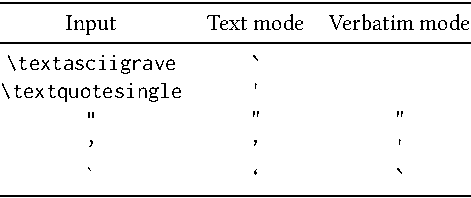
\includegraphics{novarqu-crop}
\end{center}
\textbf{Without \texttt{varqu}, \texttt{noupquote}:} \texttt{upquote} NOT loaded---all encodings render the same.
\begin{center}
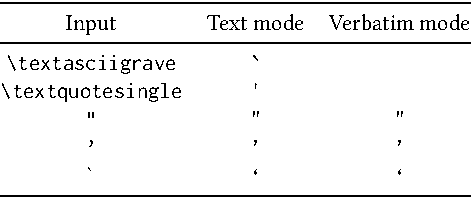
\includegraphics{novarqu-noupq-crop}
\end{center}
\textbf{With \texttt{varqu}, \texttt{noupquote}:} \texttt{upquote} NOT loaded---all encodings render the same.
\begin{center}
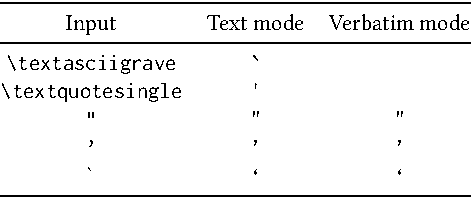
\includegraphics{novarqu-noupq-crop}
\end{center}


\textbf{Conclusion:} To me, it is overwhelmingly clear that the best results come from
specifying the option \texttt{varqu}, not specifying \texttt{noupquote}, and avoiding the QX encoding wherever  possible.

\textbf{A technical note concerning LY1 or QX encodings:} These encodings make their own definitions of \verb|\textquotesingle| as glyphs in the main text font. Using the TS1 glyph with upright shape so that \texttt{upquote} works correctly with these encodings requires the incantation:
\begin{verbatim}
\UndeclareTextCommand{\textquotesingle}{LY1} % or QX
\DeclareTextSymbol{\textquotesingle}{TS1}{39}
\usepackage{upquote}
\end{verbatim}
which is built-in to the \texttt{zi4.sty} code and need not be repeated.
\section{Opentype issues} The package includes two Opentype fonts named \textsf{Inconsolatazi4-Regular} and \textsf{Inconsolatazi4-Bold}, which may be loaded with \texttt{fontspec}:
\begin{verbatim}
\fontspec{Inconsolatazi4} %slashed zero, curly quotes, default l
\end{verbatim}
The fonts contain three Stylistic Set variants that may be used to control the shape of lower case l (\texttt{ss01}), the form of zero (\texttt{ss02}) and the shape of quotes (\texttt{ss03}). One or more of these may be specified as follows:
\begin{verbatim}
\textsf[StylisticSet=1]{Inconsolatazi4-Regular} % shapely l
\end{verbatim}
\begin{verbatim}
\textsf[StylisticSet=2]{Inconsolatazi4-Regular} % unslashed zero
\end{verbatim}
\begin{verbatim}
\textsf[StylisticSet=3]{Inconsolatazi4-Regular} % straight quotes
\end{verbatim}
\begin{verbatim}
\textsf[StylisticSet={1,3}]{Inconsolatazi4-Regular} % shapely l, upright quotes
\end{verbatim}
Note that one cannot expect exactly the same rendition from \LaTeX\ typewriter modes and the \textsf{fontspec} typewriter modes. For one thing, in \LaTeX, the typewriter left quote symbol is \texttt{quoteleft}, while under \textsf{fontspec}, it is the \texttt{grave} symbol.
\end{document}



 